\chapter{电流强度与电流表}\label{ch:g8:intensity-ammeter}

“强电流，弱电流”——我们多年来一直这样说，
全凭感觉调节亮度与握力。今天起，感觉退休了。
电流的强弱有了名称、单位和测量仪器；
而这台仪器证明的第一条规律，
你早已隐约怀疑，却从未亲手测过。

\section{电流强度及其单位}

\begin{definition}[电流强度]\label{def:g8:intensity-ammeter:intensity}
\emph{电流强度}\index{电流强度} $I$ 衡量电流的强弱，
即每秒有多少电荷穿过电路中的某一点，
也就是电流的“流量”，正如河流的流量是每秒流过的水量。
其单位是
\emph{安培}\index{安培}（\unit{A}），以纪念一位电学先驱；
日常电路中常用
\emph{毫安}作单位：$\qty{1}{mA} = \qty{0.001}{A}$，
即千分之一安。
\end{definition}

\begin{example}[常见电流的大小]\label{ex:g8:intensity-ammeter:values}
一只小指示灯耗电约 \qty{0.02}{A} ——
即 \qty{20}{mA}；手电筒灯泡约 \qty{0.3}{A}；汽车前大灯为
\qty{5}{A}；满功率运转的电热水壶为
\qty{10}{A}；汽车启动时，发动机从蓄电池中吸取 \qty{100}{A}；
一次闪电击中，历时仅一毫秒，却有数万
安培的电流沿其通道猛冲而下。危险的尺度
同样发人深省：几百分之一安培的电流穿过人体，
就足以致命——对电流的敬畏，
远在一安培之前就该开始。
\end{example}

\begin{remark}[人名与单位]\label{rem:g8:intensity-ammeter:person}
写出来时，单位名称用小写，如“两安培的电流”，
而大写的则是那位科学家的名字，
与所有以科学家命名的单位一样；符号 \unit{A} 保持大写。
这一约定很快还会再遇到两次。
\end{remark}

\section{电流表}

\begin{definition}[电流表]\label{def:g8:intensity-ammeter:ammeter}
\emph{电流表}\index{电流表}用来测量电流强度，它计量
流经\emph{自身}的电流，因此必须
\emph{串联}接入所测量的回路之中，如同
公路上的收费站。为尽量少扰动电流，
它几乎不阻碍电流——这也
正是电流表若被错误地直接跨接在电池两端，
就成了一个带表盘的短路：这是烧坏电流表的经典做法。
\end{definition}

\begin{method}[测量电流强度]\label{met:g8:intensity-ammeter:measure}
\begin{enumerate}
  \item 关闭电路开关，在待测电流所在处
        \emph{断开}回路；
  \item 将电流表接入缺口：电流由其
        \unit{A} 接线柱流入，由\emph{公共}接线柱流出，
        使电流的规定方向从电表的
        “正门”进入；
  \item 若为多量程电表，先选用\emph{最大}量程，
        再逐级调小，直至读数舒适地落在表盘上，
        以保护电表免受
        意外损坏；
  \item 闭合开关，读数，并写上单位。
\end{enumerate}
若指针式电表接反，指针会猛撞在限位上；
数字式电表则只显示一个负号，
天天宽容着学生的粗心。
\end{method}

\begin{omfigure}
\begin{tikzpicture}[scale=0.9]
  \draw (0,0) to[battery1, l=battery] (0,2.8)
    to[short] (1.8,2.8)
    to[ammeter, l=$I$] (4.2,2.8)
    to[lamp, l=lamp] (6.6,2.8)
    to[short] (8.0,2.8)
    to[short] (8.0,0)
    to[short] (0,0);
  \draw[-Stealth, very thick, omThm] (1.0,3.15) -- (1.7,3.15);
\end{tikzpicture}

{\small 电流表在回路中占据自己的位置：如同串联在回路中的收费站，
计量着点亮灯泡的那股电流。}
\end{omfigure}

\begin{omfigure}
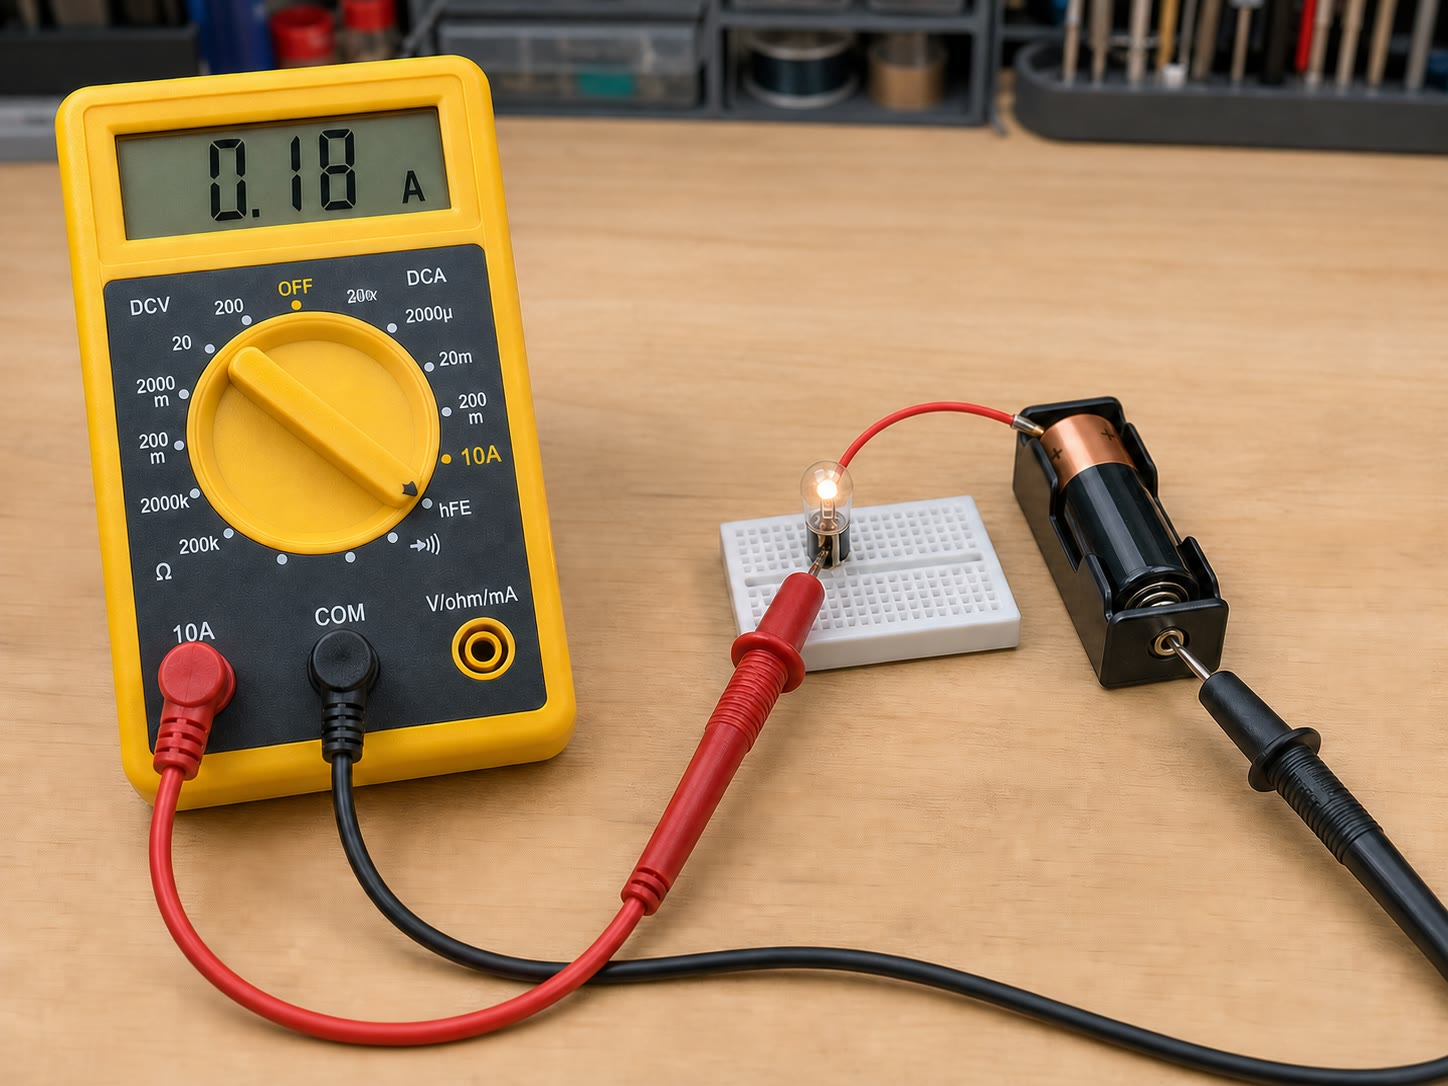
\includegraphics[width=0.5\linewidth]{images/book1/ai/g8-ammeter-multimeter.jpg}

{\small 实验台上的实物：一台仪器、两根表笔，电路中的电流便在显示屏上变为一个数字。}
\end{omfigure}

\section{第一条被测定的规律}

\begin{proposition}[同一回路，同一强度]\label{prop:g8:intensity-ammeter:sameI}
在串联电路中，回路上各点的电流强度都相同。
将电流表移至任意位置——灯泡之前、之后，
或紧靠电池，读数都不会改变。
五年来亮度相同的灯泡所暗示的结论，
如今电表以数值予以确认：途中并无电流被消耗；
一条路，一股电流，一个 $I$。
\end{proposition}

\begin{omfigure}
\begin{tikzpicture}[scale=0.85]
  \draw (0,0) to[battery1] (0,3.0)
    to[ammeter, l=\qty{0.30}{A}] (2.6,3.0)
    to[lamp] (4.8,3.0)
    to[ammeter, l=\qty{0.30}{A}] (7.4,3.0)
    to[lamp] (9.6,3.0)
    to[short] (9.6,0)
    to[ammeter, l=\qty{0.30}{A}] (4.8,0)
    to[short] (0,0);
\end{tikzpicture}

{\small 同一回路上的三个收费站：灯泡之前、灯泡之间和灯泡之后，
每个电流表都显示同样的 \qty{0.30}{A}。}
\end{omfigure}

\begin{example}[读懂定律的细则]\label{ex:g8:intensity-ammeter:fineprint}
定律说的是\emph{沿同一回路}，而不是\emph{对回路做的任何改动}。
若再串联一只灯泡，电流整体减弱，
比如从 \qty{0.30}{A} 降到
\qty{0.17}{A}，但处处都\emph{同等}地减弱；
三个收费站在新数值上也一致。
同一回路，同一电流强度——无论它此刻是多少。
\end{example}

\begin{example}[一瞥节点]\label{ex:g8:intensity-ammeter:junction}
改为在一对并联支路上设置收费站：干路
\qty{0.50}{A}；支路一 \qty{0.30}{A}；支路二
\qty{0.20}{A}。这个颇具启发性的和并非偶然——电流
流入和流出节点的电流必须平衡，因为电荷
在分叉路口既不会凭空产生，也不会凭空消失。完整的定律
连同与之对应的电压定律，
将在隔一章的内容中详述；你的电表其实早已接触过它。
\end{example}

\begin{remark}[万用表]\label{rem:g8:intensity-ammeter:multimeter}
车间里那块黄色的“砖头”——\emph{万用表}——把
电流表和其他几种仪器合并到一个机身里，靠
一个选择旋钮切换。旋钮拨到 \unit{A} 或 \unit{mA} 档，表笔插入
标有记号的插孔，它就是你的电流表，串联规则照样适用。
本书已有两章内容藏在其中；下一章还将引入第三类
，注意它的接线规则与之\emph{相反}。
\end{remark}

\section{练习}

\begin{exercise}[$\star$]\label{exo:g8:intensity-ammeter:1}
用“河流”的比喻来说，电流强度测量的是什么？写出它的单位
和符号，并将 \qty{250}{mA} 换算为安培。
\end{exercise}

\begin{exercise}[$\star$]\label{exo:g8:intensity-ammeter:2}
将电流强度与对应场景配对：\qty{0.02}{A}；\
\qty{0.3}{A}；\ \qty{10}{A}；\ \qty{100}{A}——
分别对应电热水壶、指示灯、启动发动机、手电筒灯泡。
\end{exercise}

\begin{exercise}[$\star$]\label{exo:g8:intensity-ammeter:3}
为什么电流表必须串联接入？它的设计目的是
几乎不阻碍电流，这会使
什么样的事故成为可能？
\end{exercise}

\begin{exercise}[$\star$]\label{exo:g8:intensity-ammeter:4}
列出正确测量电流强度的四个步骤。为什么
要从最大量程开始？
\end{exercise}

\begin{exercise}[$\star$]\label{exo:g8:intensity-ammeter:5}
叙述“同一回路，同一电流强度”的定律。它把哪一个以前的
“亮度相同”的观察结果变成了数值？
\end{exercise}

\begin{exercise}[$\star$]\label{exo:g8:intensity-ammeter:6}
一只电流表位于串联电动机之前，读数为 \qty{0.45}{A}。
电动机之后它读数是多少？电池旁边的读数又是多少？
\end{exercise}

\begin{exercise}[$\star$]\label{exo:g8:intensity-ammeter:7}
在串联回路中再接入一只灯泡后，电流表的读数
由 \qty{0.30}{A} 变为 \qty{0.17}{A}。定律是否失效？
请解释其中的细则。
\end{exercise}

\begin{exercise}[$\star$]\label{exo:g8:intensity-ammeter:8}
一只数字电流表的读数为 $-0.25$ \unit{A}。该学生做了什么？
这一错误有多严重？
\end{exercise}

\begin{exercise}[$\star\star$]\label{exo:g8:intensity-ammeter:9}
干路 \qty{0.60}{A}；支路一 \qty{0.35}{A}。支路二
中的电流是多少？依据什么推理？第二个节点的
收费站读数是多少？
\end{exercise}

\begin{exercise}[$\star\star$]\label{exo:g8:intensity-ammeter:10}
一名学生把电流表与灯泡\emph{并联}连接，
“为了比较它们”。请预测两个后果——对灯泡和对电流表——
并指出学生无意中
搭建出的“罪魁祸首”。
\end{exercise}

\begin{exercise}[$\star\star$]\label{exo:g8:intensity-ammeter:11}
两只相同的灯泡并联，每只通过 \qty{0.30}{A}。电池的干路
电流是多少？再并联一只相同的灯泡，
请预测干路的新负担，并
指出哪一样会耗得更快。
\end{exercise}

\begin{exercise}[$\star\star\star$]\label{exo:g8:intensity-ammeter:12}
为一个两条支路（灯泡和电动机）的并联电路
设计完整的测量方案：需要多少个电流表位置，
才能得知电路中\emph{每一处}的电流；
最少测量几次即可（其中一次可由
哪一种平衡关系推出？）；以及操作的先后顺序，
使电表始终不会处于危险的接线状态。
\end{exercise}

\section{问题：计量工作台}

\begin{problem}[{周末问题——电子车间的资格考核日；
四个工位，每个工位一只电流表；
学徒的执照}]\label{pb:g8:intensity-ammeter:1}
为获得车间的操作权限，每位学徒需要巡视
四个测量工位。请带上本章内容。

\medskip\noindent\textbf{第一部分——第一站：简单
回路。}
电池、开关、一盏灯。
\begin{enumerate}
  \item 逐步描述如何接入电流表，
        以测量灯的电流。
  \item 读数为 \qty{280}{mA}。请换算为安培。
  \item 考官把你的电表移到电池的
        另一侧。请预测读数，并引用相应定律说明理由。
  \item “如果此回路中同时接两只电流表呢？”
        它们可以接在哪里？分别会显示什么？
\end{enumerate}

\medskip\noindent\textbf{第二部分——第二站：串联
对。}
两盏不同的灯，A 比 B 亮，串联连接。
\begin{enumerate}[resume]
  \item 一位学徒预测：“较亮的 A 通过的电流比较暗的 B 多。”
        请用定律检验这一预测，
        并调和电流相等与亮度不同之间的矛盾
        （两盏灯之间必须有什么不同？）。
  \item 电表在 A 与 B 之间的读数为 \qty{150}{mA}。请写出
        回路中其余每一处的电流。
  \item 灯 B 被一根导线短接。请预测
        新的读数以及两盏灯的状况。
  \item 考官要求用一句话说明，为什么车间禁止在
        \emph{电池}两端接导线短接，
        却允许在 B 两端进行此项演示。
\end{enumerate}

\medskip\noindent\textbf{第三部分——第三站：
节点。}
一条灯支路与一条电动机支路并联。
\begin{enumerate}[resume]
  \item 干路：\qty{0.52}{A}；灯支路：\qty{0.30}{A}。
        由节点平衡，电动机支路的电流为多少？
  \item 电动机卡住（仍接在电路中，但不转动），其
        支路电流升至 \qty{0.40}{A}。假设灯支路保持
        \qty{0.30}{A}，则干路现在通过多大的电流，
        哪一个车间安全装置
        正在监听？
  \item 拧下灯泡。请预测三处
        电流表的全部读数。
  \item 两条支路均正常时，电池为何耗电最快？
        电能究竟消耗在哪里？
\end{enumerate}

\medskip\noindent\textbf{第四部分——执照。}
\begin{enumerate}[resume]
  \item 写出学徒誓言，共三行：电流表应接在哪里、
        绝不能接在哪里；一个回路保证什么；
        一个节点平衡什么。
\end{enumerate}
\end{problem}
